\documentclass[a4paper, 12pt]{report}
% Allows writing the document in english.
\usepackage[francais]{babel}
% Allows to use images.
\usepackage{graphicx}
% Provides hyperlinks within the document.
\usepackage{enumitem}
% Adds space between paragraphs.
\usepackage{parskip}
% Supports Text Companion fonts (necessary for gensymb).
\usepackage{textcomp}
\usepackage{array}
\usepackage{multicol}
% Better tabular
\usepackage{tabularx}
% Allows to use colors.
\usepackage{xcolor}
\usepackage[margin=4cm]{geometry}
\usepackage{varwidth}
% Euro
\usepackage{eurosym}
\usepackage{amsmath}
\usepackage[T1]{fontenc} 
\usepackage{lmodern} 

\usepackage{minted}

\usepackage{gensymb}

% Default fixed font does not support bold face
\DeclareFixedFont{\ttb}{T1}{txtt}{bx}{n}{12} % for bold
\DeclareFixedFont{\ttm}{T1}{txtt}{m}{n}{12}  % for normal

\setcounter{tocdepth}{3}

% Custom colors
\usepackage{color}
\definecolor{deepblue}{rgb}{0,0,0.5}
\definecolor{deepred}{rgb}{0.6,0,0}
\definecolor{deepgreen}{rgb}{0,0.5,0}

\usepackage{listings}

% Python style for highlighting
\newcommand\pythonstyle{\lstset{
language=Python,
basicstyle=\ttm,
otherkeywords={self},             % Add keywords here
keywordstyle=\ttb\color{deepblue},
emph={MyClass,__init__},          % Custom highlighting
emphstyle=\ttb\color{deepred},    % Custom highlighting style
stringstyle=\color{deepgreen},
frame=tb,                         % Any extra options here
showstringspaces=false            %
}}


% Python environment
\lstnewenvironment{python}[1][]
{
\pythonstyle
\lstset{#1}
}
{}

% Python for external files
\newcommand\pythonexternal[2][]{{
\pythonstyle
\lstinputlisting[#1]{#2}}}

% Python for inline
\newcommand\pythoninline[1]{{\pythonstyle\lstinline!#1!}}

\usepackage{subfigure}
\usepackage[
    type={CC},
    modifier={by-nc-nd},
    version={4.0},
]{doclicense}

\usepackage[colorlinks=true,urlcolor=black,linkcolor=black]{hyperref}
% New columns types
% Left
\newcolumntype{L}{>{\raggedright\arraybackslash}X}
% Center
\newcolumntype{C}{>{\centering\arraybackslash}X}
% Right
\newcolumntype{R}{>{\raggedleft\arraybackslash}X}

% Add more space before and after table
\newenvironment{centerspace}{\setlength{\topsep}{1ex}\center}{\endcenter}
% Sets the color of gray.
\newcommand{\gray}{\rowcolor[gray]{.90}}
% Allows to draw lines.
\newcommand{\HRule}{\rule{\linewidth}{0.5mm}}
% Uses the arabic numerals for sections.
\renewcommand{\thesection}{\arabic{section}}

% Width of text.
\addtolength{\textwidth}{2cm}
% Odd page left margin.
\addtolength{\oddsidemargin}{-1cm}
% Height of main text.
\addtolength{\textheight}{2cm}
% Removes indentation.
\setlength\parindent{0pt}
% Indicates overflow words.
\setlength{\overfullrule}{10pt}
% Height of items.
\setitemize{itemsep=1em}

%%%%********************************************************************
% fancy quotes
\definecolor{quotemark}{gray}{0.7}
\makeatletter
\def\fquote{%
    \@ifnextchar[{\fquote@i}{\fquote@i[]}%]
           }%
\def\fquote@i[#1]{%
    \def\tempa{#1}%
    \@ifnextchar[{\fquote@ii}{\fquote@ii[]}%]
                 }%
\def\fquote@ii[#1]{%
    \def\tempb{#1}%
    \@ifnextchar[{\fquote@iii}{\fquote@iii[]}%]
                      }%
\def\fquote@iii[#1]{%
    \def\tempc{#1}%
    \vspace{1em}%
    \noindent%
    \begin{list}{}{%
         \setlength{\leftmargin}{0.1\textwidth}%
         \setlength{\rightmargin}{0.1\textwidth}%
                  }%
         \item[]%
         \begin{picture}(0,0)%
         \put(-15,-5){\makebox(0,0){\scalebox{3}{\textcolor{quotemark}{``}}}}%
         \end{picture}%
         \begingroup\itshape}%
 %%%%********************************************************************
 \def\endfquote{%
 \endgroup\par%
 \makebox[0pt][l]{%
 \hspace{0.8\textwidth}%
 \begin{picture}(0,0)(0,0)%
 \put(15,15){\makebox(0,0){%
 \scalebox{3}{\color{quotemark}''}}}%
 \end{picture}}%
 \ifx\tempa\empty%
 \else%
    \ifx\tempc\empty%
       \hfill\rule{100pt}{0.5pt}\\\mbox{}\hfill\tempa,\ \emph{\tempb}%
   \else%
       \hfill\rule{100pt}{0.5pt}\\\mbox{}\hfill\tempa,\ \emph{\tempb},\ \tempc%
   \fi\fi\par%
   \vspace{0.5em}%
 \end{list}%
 }%
 \makeatother

 %%%% ********************************************************************

% Starts roman numbering (trick to not numbering the first pages).
\pagenumbering{roman}

\begin{document}
\renewcommand{\bibname}{Références}
\begin{center}
  
\includegraphics[scale=0.12]{textures/logo/heh_bw.pdf}

  \vspace{1cm}

  \textsc{\LARGE Projet} \\ [0.5cm]
  \textsc{\Large Réalisation d'un site en PHP} \\ [0.5cm]

  \textsc{\large 2\up{ème} Bachelier en Informatique} \\ [0.2cm]

  \begingroup
  \fontfamily{pag} \selectfont 

  \HRule \\ [0.4cm] {
    \huge Programmation web \\ [0.2cm] 
  }
  \HRule \\ [1.3cm]
  \endgroup
  \begin{minipage}[t]{0.4 \textwidth} 
    \begin{flushleft} 
      \large \emph{Auteur:} \\ 
      Alexandre \textsc{Ducobu}
    \end{flushleft} 
  \end{minipage}
  % 
  \begin{minipage}[t]{0.4 \textwidth}
    \begin{flushright} 
      \large \emph{Enseignants :} \\ 
      Antoine \textsc{Malaise} \\
      Fabrice \textsc{Scopel}
    \end{flushright} 
  \end{minipage}

  \vspace{1cm}

  
\includegraphics[scale=0.08]{textures/logo/technical_bw.pdf}

  \vspace{0.5cm}

  Année académique 2016 - 2017
\end{center}

\thispagestyle{empty}

\newpage
\newpage
\thispagestyle{empty}
\setcounter{page}{0}
\null
\newpage
\begin{center}
  
\includegraphics[scale=0.12]{textures/logo/heh.pdf}

  \vspace{2cm}

  \textsc{\LARGE Projet ARS} \\ [0.5cm]
  \textsc{\Large Les différents systèmes d'exploitation} \\ [0.5cm]

  \textsc{\large 1er Bachelier en Informatique} \\ [0.2cm]
  \textsc{Groupe 5-8} \\

  \begingroup
  \fontfamily{pag} \selectfont 

  \HRule \\ [0.4cm] {
    \huge Architecture des Systèmes II \\ [0.2cm] 
  }
  (Laboratoire)
  \HRule \\ [1.3cm]
  \endgroup

  \begin{minipage}[t]{0.4 \textwidth} 
    \begin{flushleft} 
      \large \emph{Auteur:} \\ 
      Agozzino \textsc{Terencio} 
    \end{flushleft} 
  \end{minipage}
  % 
  \begin{minipage}[t]{0.4 \textwidth}
    \begin{flushright} 
      \large \emph{Auteur :} \\ 
      Ducobu \textsc{Alexandre} 
    \end{flushright} 
  \end{minipage}

  \vspace{0.5cm}

  \begin{minipage}[t]{0.4 \textwidth}
    \begin{center} 
      \large \emph{Enseignant:} \\ 
      Desmet \textsc{Erwin} 
    \end{center} 
  \end{minipage}

  \vspace{0.5cm}

  
\includegraphics[scale=0.08]{textures/logo/technical.pdf}

  \vspace{0.5cm}

  Année académique 2015 - 2016
\end{center}

\thispagestyle{empty}

\newpage
\newpage
\thispagestyle{empty}
\setcounter{page}{0}
\null
\newpage
\newpage
\mbox{~}
\vfill
\hfill
\begin{tabular}{@{}l@{}}
  Nous remercions en particulier \\
  Monsieur David ARNAUD de nous \\
  avoir permis d'utiliser le matériel \\
  en dehors des heures de laboratoire. \\ \\

  Ainsi que Monsieur Florian DI VRUSA \\
  pour nous avoir indiqué une erreur \\
  au niveau de la prise en charge de \\
  la librairie Sense HAT en Python.
\end{tabular}
\setcounter{page}{0}
\thispagestyle{empty}
\newpage
\mbox{~}
\vfill
Ce document est mis à disposition selon les termes de la licence Creative
Commons ``\href{https://creativecommons.org/licenses/by-nc-nd/4.0/}{Attribution -
Pas d'utilisation commerciale 4.0 International}''.

\begin{figure}[!h]
  \centering
  
\includegraphics[width=0.25\textwidth]
  {textures/images/license/license.eps}
\end{figure}

\thispagestyle{empty}

\newpage
\pagenumbering{arabic}
\tableofcontents
\newpage
\section{Présentation du projet}
\label{sec:presentation}


\subsection{Introduction}
\label{subsec:intro}

Dans le cadre du cours de \textbf{Gestion de projets}, il nous a été demandé de réaliser un projet au choix individuellement ou par deux. J'ai choisi de le faire seul. \\
En effet, nous avons déjà d'autres travaux de groupes. Je trouve donc qu'un travail individuel est un plus dans notre cursus scolaire. \\
Lors des deux premières séances de laboratoire, chaque groupe a rédigé une fiche descriptive du projet, avec l’enseignant, afin de baliser le travail à effectuer durant l’année.\\
Lors de ces séances, l’enseignant a validé chacun des projets.


\subsection{But}
\label{subsec:but}

Grâce à ce projet, nous allons apprendre à gérer nos projets à l'aide de différents outils spécialisés tels que \textbf{\textit{Microsoft Project}}, \textit{le diagramme de \textbf{Gantt}} et \textit{le graphique de \textbf{PERT}}.\\
Ceux-ci nous aideront dans la planification de notre projet ainsi que, pour les binômes, dans la répartition des tâches. 


\subsection{Choix du projet}
\label{subsec:choix}

Ce projet, \textit{un site web}, permettra d'apprendre les bases de la programmation en \textit{Python} et sera divisé en chapitres: les variables, les conditions, les boucles, les tableaux, etc.\\

L’apprentissage se fera en trois étapes:
\begin{enumerate}
    \item L’utilisateur découvrira le nouveau sujet par de la théorie ainsi que par un ou plusieurs exemples. Il en apprendra alors l’utilité et le fonctionnement.
    \item Entre deux parties théoriques, l’utilisateur mettra en pratique ce qu’il aura appris au travers de petits QCM.
    \item Une fois le chapitre terminé, un questionnaire (QCM, ordonnancement du code,...) sera proposé à l’utilisateur.\\
    Celui-ci sera noté sur 10 afin que l’utilisateur puisse se juger et s’améliorer.\\
    Le passage au chapitre suivant requerra une \textit{cote minimale de 7/10}.\\
\end{enumerate}

D'autre part, ce projet sera un pré-TFE.\\
À terme, il sera possible de créer facilement des cours et de s’y inscrire.\\ Il pourra être utilisé aussi bien par les écoles que par  \og \textit{les particuliers} \fg.


%%% Local Variables:
%%% mode: latex
%%% TeX-master: t
%%% End:

\newpage
\section{Choix}
\label{sec:choix}

\subsection{Langage}
\label{sec:langage}

Pour ce projet, notre choix s'est naturellement porté vers le Python.
En effet, en plus d'être le langage de prédilection sur le Raspberry Pi, il dispose d'une
documentation et d'une vaste communauté. \\
En outre, ce langage apporte une facilité pour l'interaction avec les
GPIO \footnote{General-purpose input/output} de la Raspberry Pi et la librairie du
Sense HAT.

\subsection{Raspbian}
\label{sec:raspbian}

Pour notre utilisation, Raspbian, étant le choix suggéré par le constructeur, a été choisi.

\begin{figure}[!h]
  \centering
  
\includegraphics[scale=0.06]
  {textures/images/choices/raspbian.pdf}
  \caption{Logo Raspbian}
  \label{fig:raspbian}
\end{figure}

\subsection{Outils de développement}
\label{sec:outils-de-devel}

GNU Emacs et Atom ont été les seuls éditeurs de texte utilisés comme outils de
développement pour leur simplicité ainsi que pour notre familiarité avec ceux-ci.

\begin{figure}[!h]
\centering
\begin{minipage}[c]{0.4\textwidth}
  \centering
  
\includegraphics[scale=0.09]
  {textures/images/choices/emacs.pdf}
\caption{Logo Emacs}\label{emacs}
\end{minipage} \qquad
\begin{minipage}[c]{0.4\textwidth}
  \centering
  
\includegraphics[scale=0.09]
  {textures/images/choices/atom.pdf}
\caption{Logo Atom}\label{atom}
\end{minipage}
\end{figure}

De plus, nous avons utilisé GitHub qui est un service en ligne permettant
d'héberger notre projet et de ce fait, synchroniser notre travail.

\begin{figure}[!h]
  \centering
  
\includegraphics[scale=0.1]
  {textures/images/choices/github.pdf}
  \caption{Logo GitHub}
  \label{fig:github}
\end{figure}

%%% Local Variables:
%%% mode: latex
%%% TeX-master: t
%%% End:
\newpage
\section{Algorithmes de programmation}
\label{sec:algor-de-progr}

\subsection{Organigramme du Pong}
\label{sec:organigramme}

\begin{figure}[!h]
  \centering
  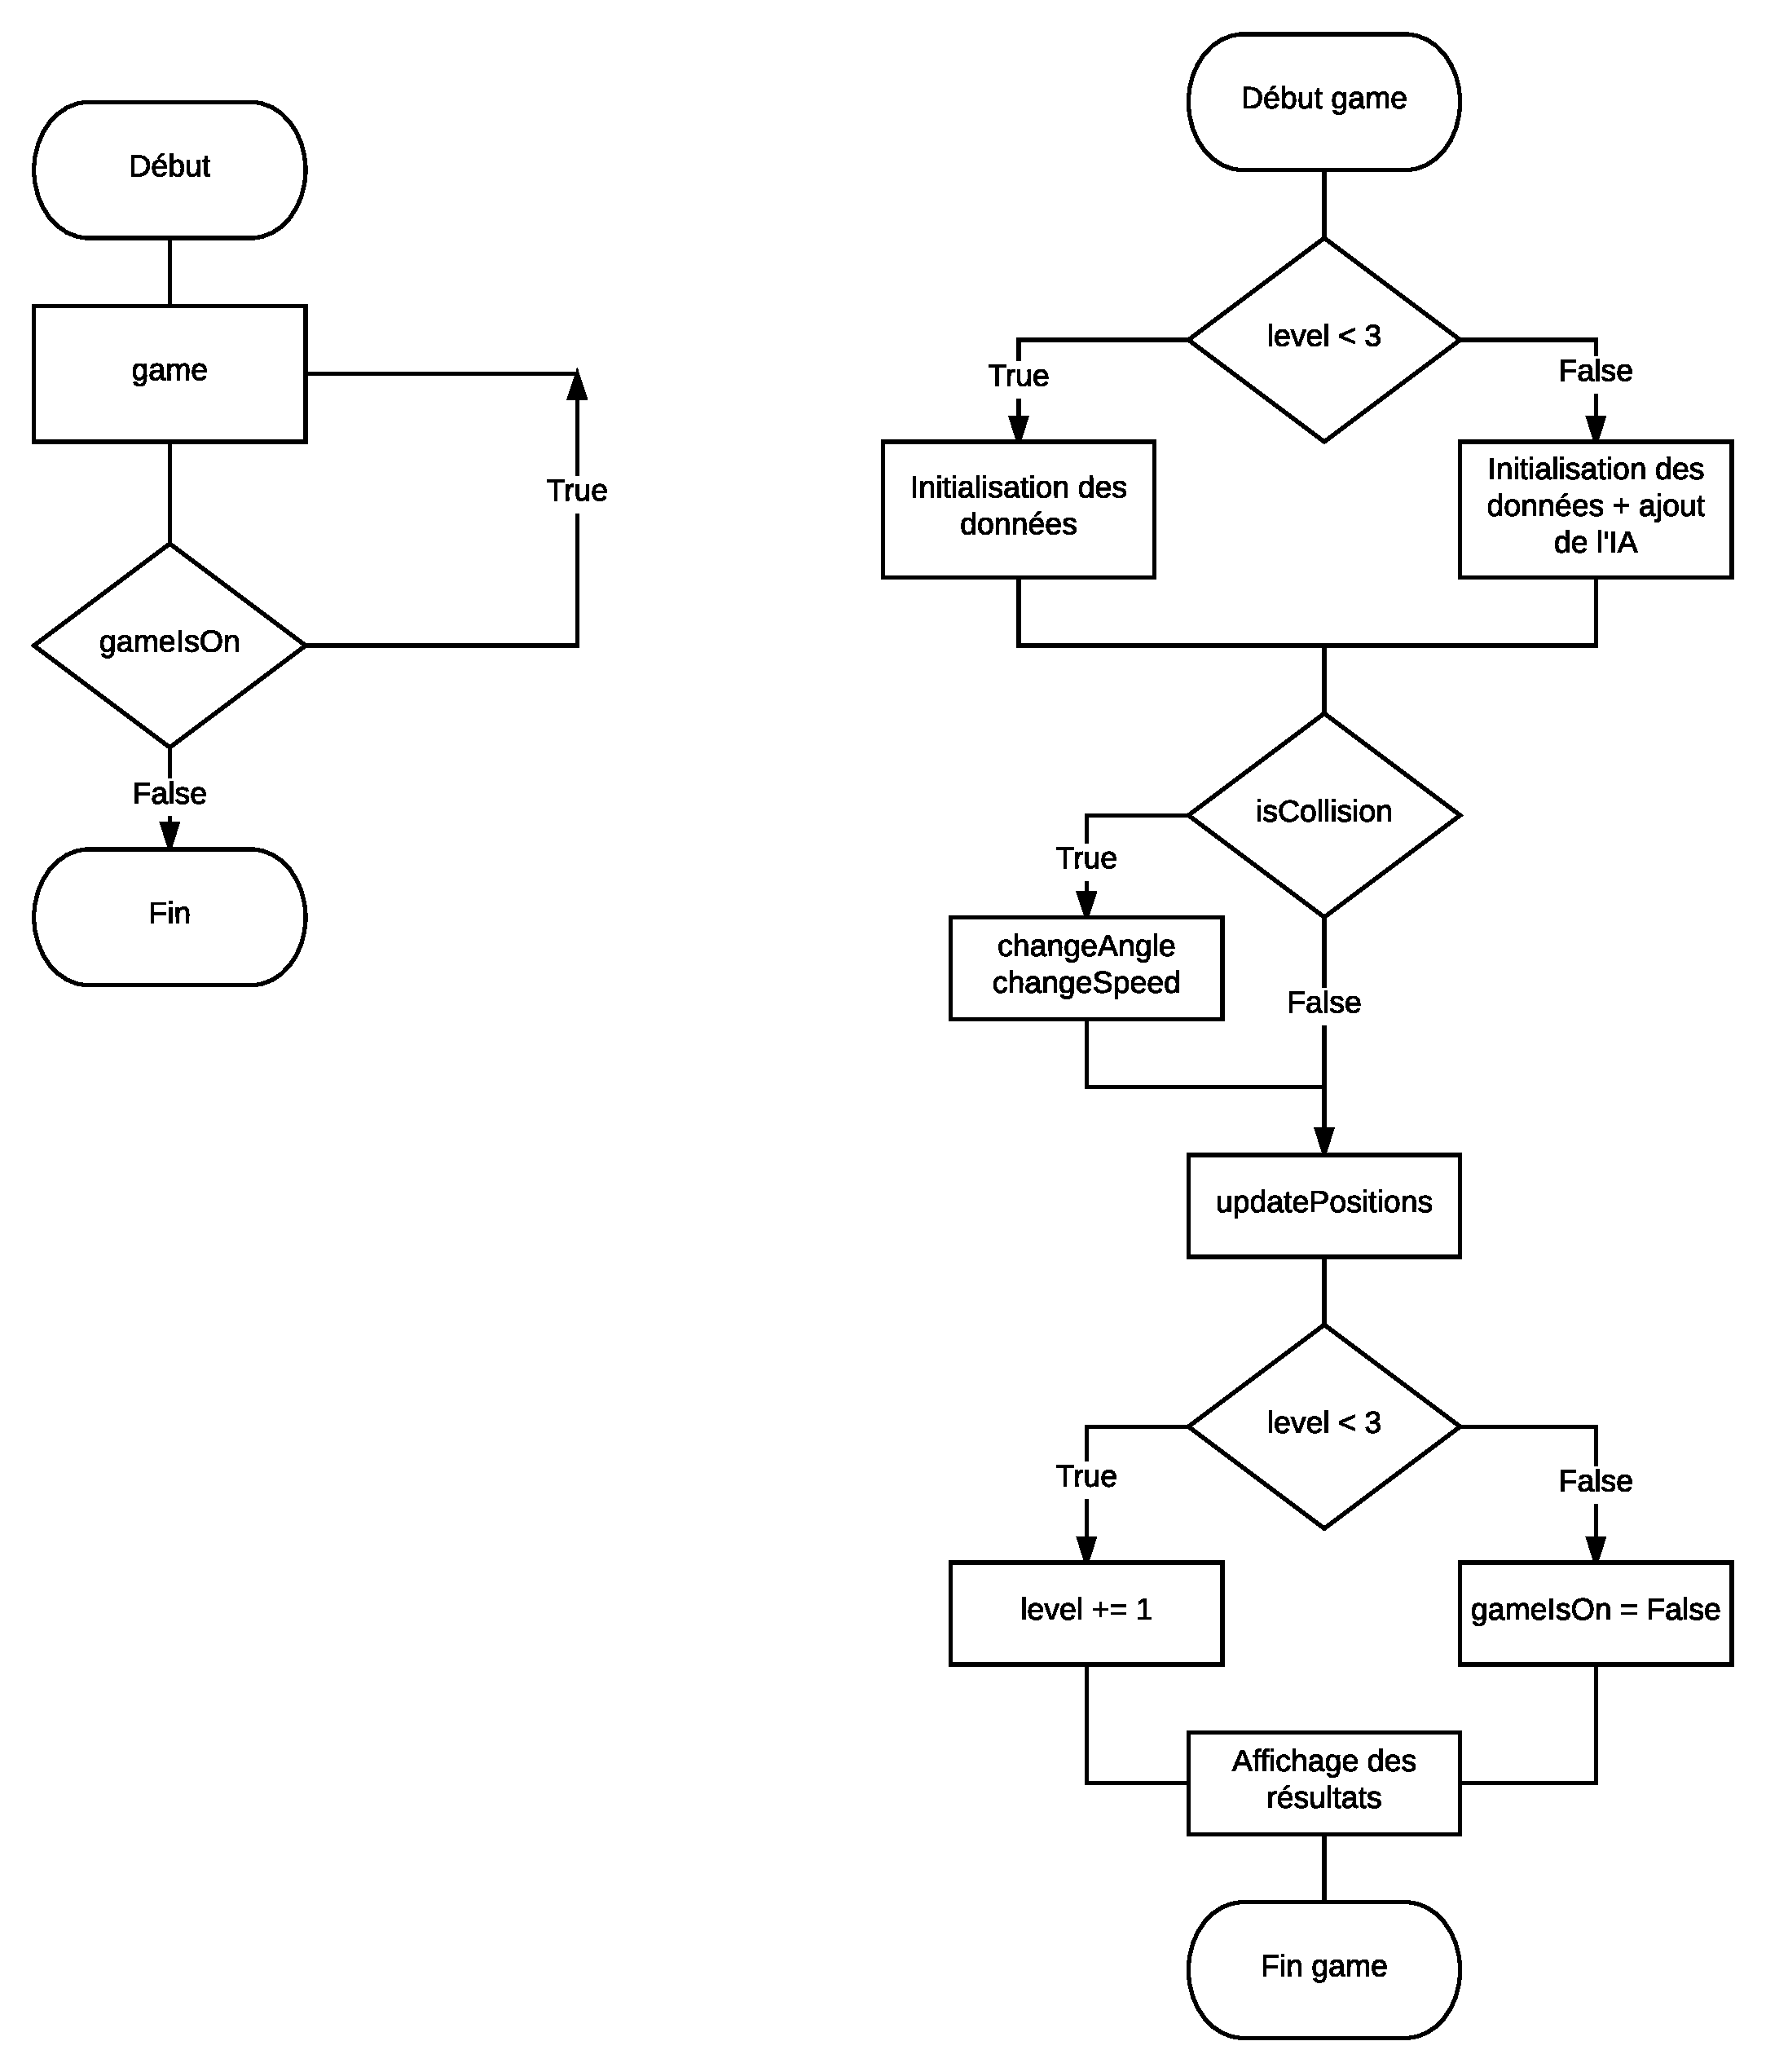
\includegraphics[scale=0.4]
  {textures/images/algorithm/organigram.pdf}
  \caption{Organigramme du PyPong}
  \label{fig:organigram}
\end{figure}

\newpage

\subsection{Collisions en détails}
\label{sec:collisions-details}

Dans ce point, il sera question de détailler le code de détection des différentes
collisions du Pong. Liée à cela, la gestion des angles sera aussi explicitée.

Pour débuter, nous avons choisi - \textit{au début du projet} - de définir le
référentiel d'après la balle. Pour elle, l'axe des abscisses est l'axe sur lequel
les raquettes se déplacent.

\subsubsection{Collision avec les murs}
\label{sec:collision-murs}

\begin{minted}{Python}
def isWallCollision(self):
    if self.level < 3:
        if self.ball.x == 0 or self.ball.x == self.row - 1:
            #Roof
            self.ball.dx = -self.ball.dx
            self.result += 3
            self.ball.speed -= 0.1
        if self.ball.y == 0:
            #Left side
            self.ball.dy = -self.ball.dy
            self.result += 3
            self.ball.speed -= 0.1
    else:
        if self.ball.x == 0 or self.ball.x == self.row - 1:
            #Roof
            self.ball.dx = -self.ball.dx
            self.ball.speed -= 0.1
\end{minted}

Dans ce cas, deux cas sont possibles: soit on est dans un des deux premiers
niveaux et on joue seul contre le mur de gauche, soit on joue contre
l'intelligence artificielle.

\begin{itemize}

    \item Prenons le premier cas, la balle peut donc rebondir sur trois surfaces: celle du
    haut, celle du bas et celle de la gauche.

    \item Prenons le second cas où la balle ne peut rebondir que sur les bords
    supérieurs et inférieurs.

\end{itemize}

La collision avec le haut ou le bas se fait respectivement quand la position
\textbf{x} est soit nulle, soit la dernière position possible dans les limites
de la grille.\\
La collision avec le mur gauche se fait de manière similaire, mais seulement
lorsque la position \textbf{y} est nulle que la balle entre en collision avec le
mur. \\

Lors d'une collision, la vitesse et le résultat sont augmentés, et la direction
\textbf{x} ou \textbf{y} est inversée. \\
Dans le cas où la balle va dans un coin gauche, elle subit les deux collisions:
le joueur gagne le double de points et la vitesse est encore plus rapide.

\newpage

\subsubsection{Collision avec les raquettes}
\label{sec:collision-raquettes}

\begin{minted}{Python}
def isPaddleCollision(self):
    if self.level < 3:
        if self.ball.y == self.column - 2 and
        self.ball.x == self.paddle.x:
            self.ball.dy = -self.ball.dy
            self.result += 2
            self.ball.speed -= 0.15
    else:
        if (self.ball.y == 1 and
        self.ball.x == self.paddleLeft.x) or
        (self.ball.y == self.column - 2 and
        self.ball.x == self.paddleRight.x):
            self.ball.dy = -self.ball.dy
            self.ball.speed -= 0.15
\end{minted}

Deux cas sont à nouveaux possibles: si le joueur se retouve contre
l'intelligence artificielle, alors il y a deux raquettes en jeu. Sinon, la balle
ne peut rebondir que sur la raquette de droite.

\begin{itemize}

    \item Dans le cas sans l'intelligence artificielle, il suffit que la balle
    soit aux coordonnées de la raquette pour qu'il y ait une collision. \\
    Lors de la collision, le résultat est augmenté de 2.

    \item Dans l'autre cas, la condition change légèrement: la balle doit
    toujours se trouver dans la colonne de la raquette \textit{(la deuxième à
    gauche ou l'avant-dernière à droite)}, et à la ligne de la bonne raquette
    \textit{(respectivement la gauche ou la droite)}.

\end{itemize}

S'il y a une collision avec une raquette, seule la direction \textbf{y} est
inversée dans le but de garder des angles à 45$^{\circ}$, et l'accélération est
légèrement supérieure à celle observée lors de la collision avec un mur.

\newpage

\subsubsection{Sortie des limites}
\label{sec:sorties-limites}

\begin{minted}{Python}
def isOut(self):
    if self.level < 3:
        return self.ball.y == self.column - 1
    return self.ball.y == 0 or self.ball.y == self.column - 1
\end{minted}

Cette méthode est très simple. \\
Comme pour les autres collisions, il y aura le cas du niveau 3, et celui des
niveaux inférieurs.

\begin{itemize}

    \item Pour le niveau 3, la balle sort de la grille de jeu si elle touche
    le bord gauche ou le bord droit \textit{(soit la première colonne, soit
    la dernière)}.

    \item Pour les autres niveaux, la balle pouvant, \textit{(devant)}, rebondir
    sur le bord de gauche, seule une collision sur le bord droit est vue comme
    une sortie hors de la grille.

\end{itemize}

%%% Local Variables:
%%% mode: latex
%%% TeX-master: t
%%% End:

\newpage
\section{Problèmes rencontrés}
\label{sec:probl-renc}

\subsection{Joystick}
\label{sec:joystick}

La librairie de python comportait une erreur dans la prise en charge du joystick
\footnote{\href{https://www.element14.com/community/community/raspberry-pi/raspberry-pi-accessories/blog/2017/01/23/raspberry-pi-sense-hat-enabling-the-joystick}{https://www.element14.com/}}. Il
a fallu supprimer les fichiers d'extension \og \textit{.py} \fg relatifs au
Sense HAT et télécharger les fichiers mis à jour.

Pour terminer, il était nécessaire de supprimer un point mal placé dans l'une des
importations de librairies.

\subsection{Matrice}
\label{sec:matrice}

Étant donné la taille du Raspberry Pi, la matrice du Sense HAT s'est avérée fort petite
pour l'implémentation du jeu de Pong traditionnel.

De ce fait, il y avait manque d'espace pour la taille des raquettes que nous
avons été obligé de limiter à une LED, tout comme pour la balle, ce qui augmente
la difficulté de prise en main du jeu.

De plus, les angles ont aussi été atteints par cette limitation matricielle, nous
empêchant d'utiliser d'autres angles que des multiples de 45.

\subsection{Gyroscope}
\label{sec:gyroscope}

Dans le cadre du projet, il nous a été demandé d'ajouter, comme fonctionnalité
supplémentaire, une version du jeu se basant sur l'utilisation du gyroscope
incorporé au Sense HAT.

Suite à un manque d'ergonomie lié à la manipulation du joystick et de
l'inclinaison du gyroscope, nous avons décidé d'implémenter une intelligence
artificielle (IA) comme autre fonctionnalité.

%%% Local Variables:
%%% mode: latex
%%% TeX-master: t
%%% End:

\newpage
\section{Possibilités futures}
\label{sec:poss-futures}

Le code étant implémenté de manière soignée et en orienté objet, celui-ci offre
beaucoup plus de possibilités pour d'éventuelles évolutions.

Lors de la conception de la version préliminaire du jeu, nous avons prévu plusieurs
évolutions possibles pour notre Pong dans le cas où nous aurions plus de temps.

En voici quelques unes:
\begin{itemize}
	\item le mouvement des raquettes sur deux axes: en plus de se déplacer sur
	l'axe vertical, les raquettes se seraient déplacées à l'horizontal.
	\item la taille des raquettes: plus le niveau serait haut, plus la raquette rapetisserait.
	\item l'ajout d'obstacles sur le terrain: des murs seraient placés de manière
	aléatoire sur le terrain pour augmenter la difficulté du jeu.
	\item les angles: avec une taille de raquette plus importante, l'implémentation de
	différents angles (50$^{\circ}$, 70$^{\circ}$, etc.) rendrait le jeu plus intéressant.
	\item la difficulté de l'IA: une seconde IA plus efficace se replacerait au centre de
	son axe dès que la balle rebondirait sur sa raquette.
\end{itemize}

%%% Local Variables:
%%% mode: latex
%%% TeX-master: t
%%% End:

\newpage
\section{Conclusion}
\label{sec:conclusion}

\subsection{Générale}
\label{sec:generale}

Ce projet nous a permis d'apprendre à utiliser le Raspberry Pi, le Sense HAT
ainsi que les nouveautés de Python 3 que nous n'avions pas encore eu la chance
d'essayer. \\
En outre, nous avons pu mieux comprendre le comportement du Sense HAT tel que
vu au cours.

Nous avons donc implémenté un jeu de Pong en Python pour le Sense HAT, en tirant
profit du joystick qui était à disposition.\\
Le jeu nous semblant \og \textit{fade} \fg, il nous est venu à l'idée de lui
rajouter un mode contre une intelligence artificielle.

Grâce à cela, nos connaissances en Python et en algorithmique ont été renforcées. \\
La prise en charge de collisions a été un challenge et un plus pour notre
expérience, car totalement inédit dans nos précédents projets. \\

Ayant perdu 8 heures sur les 20 initialement prévues à cause du manque d'énoncé
et de matériel lors des premières séances, nous avons dû nous dépasser pour
terminer le projet dans les délais. \\
Cela nous a ainsi permis de nous améliorer dans notre gestion du temps.

\newpage

\subsection{Conclusions individuelles}
\label{sec:individuelles}

 \begin{fquote}[Terencio Agozzino]Me concernant, j'ai déjà pu apprivoiser le
   langage Python à l'Université lors d'anciens projets, ainsi que pour des
   projets personnels. Néanmoins, ce projet m'a permis de manipuler un Raspberry
   Pi en fonction de l'algorithmique et prendre conscience de la complexité de
   celui-ci avec le hardware.
 \end{fquote}

 \begin{fquote}[Alexandre Ducobu]Grâce à ce projet, je me suis perfectionné en
 algorithmique par la prise en charge des angles liés aux collisions.\\
 Il y a un an, nous avions eu l'occasion de programmer un pic en C.\\
 Ce projet était ainsi une continuation m'ayant permis d'utiliser
 un Raspberry Pi, chose qui me tentait depuis plusieurs années.
 \end{fquote}

%%% Local Variables:
%%% mode: latex
%%% TeX-master: t
%%% End:

\newpage
\section{Code du projet}
\label{sec:code-project}

% To compile with minted:
% pip install Pygments and use
% - 'pdflatex -shell-escape main.tex' for pdflatex
% - 'xelatex -8bit -shell-escape main.tex' for xelatex

\subsection{AI}
\label{sec:ai}
\inputminted{python}{src/code/ai.py}

\newpage

\subsection{Ball}
\label{sec:ball}
\inputminted{python}{src/code/ball.py}

\newpage

\subsection{Component}
\label{sec:Component}
\inputminted{python}{src/code/component.py}

\newpage

\subsection{Game}
\label{sec:game}
\inputminted{python}{src/code/game.py}

\newpage

\subsection{Ground}
\label{sec:ground}
\inputminted{python}{src/code/ground.py}

\newpage

\subsection{Paddle}
\label{sec:paddle}
\inputminted{python}{src/code/paddle.py}


%%% Local Variables:
%%% mode: latex
%%% TeX-master: t
%%% End:

\newpage
\phantomsection
\nocite{*}
\addcontentsline{toc}{section}{Références}

\begin{category}{Livres}
    \SBentries{algo}
    \SBentries{cHeH}
    \SBentries{csHeH}
    \SBentries{cZero}
    \SBentries{javaZero}
    \SBentries{latex}
    \SBentries{mor}
\end{category}

\begin{category}{Internet}
    \SBentries{website:bootstrap}
    \SBentries{website:laravel}
    \SBentries{website:pythonWiki}
    \SBentries{website:pythonZero}
    \SBentries{website:slider}
    \SBentries{website:xDupre}
\end{category}

\bibliographystyle{acm} 
\bibliography{bibli}


\newpage
\newpage
\thispagestyle{empty}
\setcounter{page}{0}
\null
\newpage
\end{document}
